\documentclass{standalone}

\usepackage{tikz}
\usetikzlibrary{arrows}
\usetikzlibrary{decorations.pathmorphing,patterns}

\begin{document}

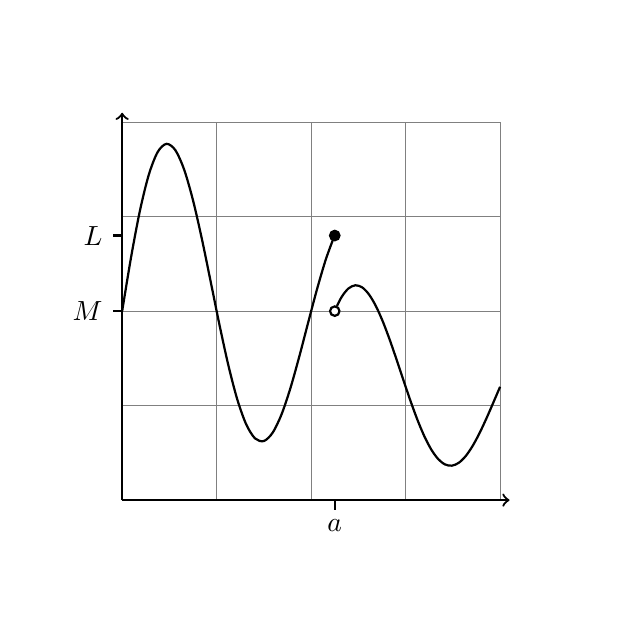
\begin{tikzpicture}[scale=1.2]%,baseline={(4,4.3)}]
  \begin{scope}[smooth,thick]
    \draw[draw=none, use as bounding box] (-1,-1) rectangle (5,5);
    \draw[color=gray,thin] (0,0) grid (4,4);
    \draw[domain=0:2.25] plot (\x,{2+2*exp(-\x/4)*sin(pi*\x r)});
    \draw[domain=2.25:4] plot (\x,{1.2+2*exp(-\x/4)*sin(pi*\x r)});
    \draw[fill] (2.25,2.8) circle(.05);
    \draw[fill,color=white] (2.25,2) circle(.05);
    \draw (2.25,2) circle(.05);
    \draw[->] (0,0) -- (4.1,0);
    \draw (2.25,0)--(2.25,-.1) node[below]{$a$};
    \draw[->] (0,0) -- (0,4.1);
    \draw (0,2.8)--(-.1,2.8) node[left]{$L$};
    \draw (0,2)--(-.1,2) node[left]{$M$};
%    \draw[fill] (.2,1.09) circle(.05);
%    \draw[fill] (3.7,2.3) circle(.05);
  \end{scope}
\end{tikzpicture}

\end{document}
